\documentclass{article}

\usepackage{longtable}
\usepackage{booktabs}
\usepackage{caption}
\usepackage{array}
\usepackage{graphicx}
\usepackage{colortbl}
\usepackage{xcolor}
\usepackage{hyperref}
\usepackage{url}
%\usepackage{fontspec}
\usepackage[english]{babel}

\usepackage{apacite}
\usepackage{lipsum}

\begin{document}



%----- Title -----

\title{\vspace{-2.0cm}

Title of the paper\\
Second line of title\footnote{\scriptsize I thank all the wonderful people in my faculty that supported my curiosity, especially X for Y.} \vspace{0.5cm}}
\author{\vspace{0.5cm}Firstname Lastname\footnote{\href{mailto:firstname.lastname@university.com}{\nolinkurl{firstname.lastnaem@university.com}}}\\
\vspace{0.5cm}\\
City School of Economics, University}
\date{\vspace{0.0cm}\footnotesize This version: \today \vspace{0.5cm}\\
\vspace{0.2cm}\footnotesize latest version: \href{https://webpage.com/paper.pdf}{click here}\vspace{-0.8cm}}


\maketitle



%----- Abstract -----

\vspace{0.3cm}
\begin{abstract}
%----- Abstract BEGIN -----
\footnotesize This paper demonstrates a collaborative workflow for reproducible science using the pipeline of writing a paper using Overleaf and editing \LaTeX-files, preparing the used tables and figures with R, and synching all together using Git.

This is a not yet a common workflow in academic research. This template shall support having reproducibility right in mind from the start of a project and serves as a template.

Furthermore, the template provides a clear and concise example of how to structure a collaborative project of this kind, including structuring a paper with sections for the introduction, literature review, data, results, conclusion, and references.\\
%----- Abstract END -----
\vspace{0.3cm}\\
\textbf{JEL-Codes:} A1, B2, C3\\
\textbf{Keywords:} Fantasy Economics, Intergalactical Trade\\
\vspace{0.3cm}
\end{abstract}

\pagebreak



%----- Introduction -----

\section{Introduction}
The purpose of this template is to allow labor distribution within a project, where some persons can focus on collaboratively write the article using Overleaf and it's conveniences, while others can work colaboratively on the data and figures using the conveniences of a version control system (Git). 

This template's structure is set up for having reproducibility in mind, right from the start of the project.

\textcolor{gray}{\lipsum[1-2]}




%----- Literature -----

\section{Literature}
This paper's theory relies on \citeA[p.123f]{smith2020economic}.

\textcolor{gray}{\lipsum[3-4]}



%----- Data -----

\section{Data}
Following \citeA{rosling2006}, this paper uses data from Gapminder \cite{gapminder}.

\textcolor{gray}{\lipsum[5]}


%----- Results -----

\section{Results}

\subsection{Figure}

In figure \ref{fig:life_expectancy} we can see the relationship between life expectancy and GDP per capita. The data shows a positive correlation, indicating that as GDP per capita increases, life expectancy tends to increase as well. This is consistent with the hypothesis that higher income levels lead to better health outcomes.
However, it is important to note that this relationship may not be causal, as other factors such as healthcare access, education, and social determinants of health also play a significant role in life expectancy.
In addition, the relationship is not linear, as there are diminishing returns to life expectancy at higher levels of GDP per capita. This suggests that while economic growth can improve health outcomes, there are limits to how much it can do so.

\begin{figure}[htbp]
\centering
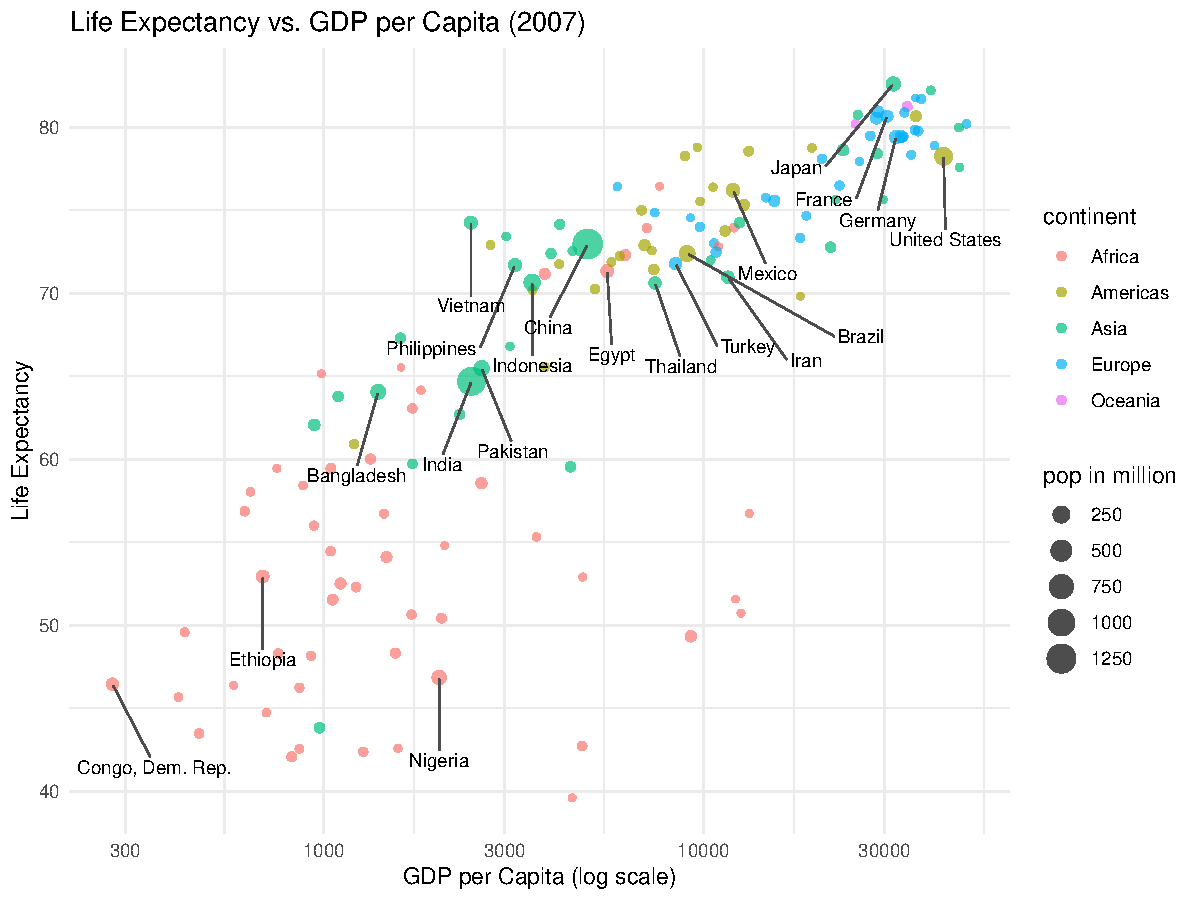
\includegraphics[width=0.9\textwidth]{../../output/figures/fig_life_expectancy.pdf}
\caption{Life Expectancy vs. GDP per Capita}
\label{fig:life_expectancy}
\end{figure}


\textcolor{gray}{\lipsum[6-8]}

\subsection{Table}

See table \ref{tab:summary-table} for a summary of the results.

\begin{table}[!t]
\caption{Summary Statistics by Continent (2007) \label{tab:summary-table}} 
\fontsize{12.0pt}{14.4pt}\selectfont
\begin{tabular*}{\linewidth}{@{\extracolsep{\fill}}crr}
\toprule
continent & mean\_lifeExp & mean\_gdpPercap \\ 
\midrule\addlinespace[2.5pt]
Africa & 54.8 & 3089.0 \\ 
Americas & 73.6 & 11003.0 \\ 
Asia & 70.7 & 12473.0 \\ 
Europe & 77.6 & 25054.5 \\ 
Oceania & 80.7 & 29810.2 \\ 
\bottomrule
\end{tabular*}
\end{table}



\textcolor{gray}{\lipsum[9-10]}



%----- Conclusion -----

\section{Conclusion}
To sum up, it is possbile to combine writing in Overleaf with the pipeline for creating figures and tables with R, synching alltogether via a version control system like Git.

\textcolor{gray}{\lipsum[11]}



%----- References -----

\section*{References}

\bibliographystyle{apacite}
\bibliography{../references/references}

\end{document}